\section{Ejemplo 8}

    \lipsum[1]
    
    \begin{figure}[h]
    	\centering
    	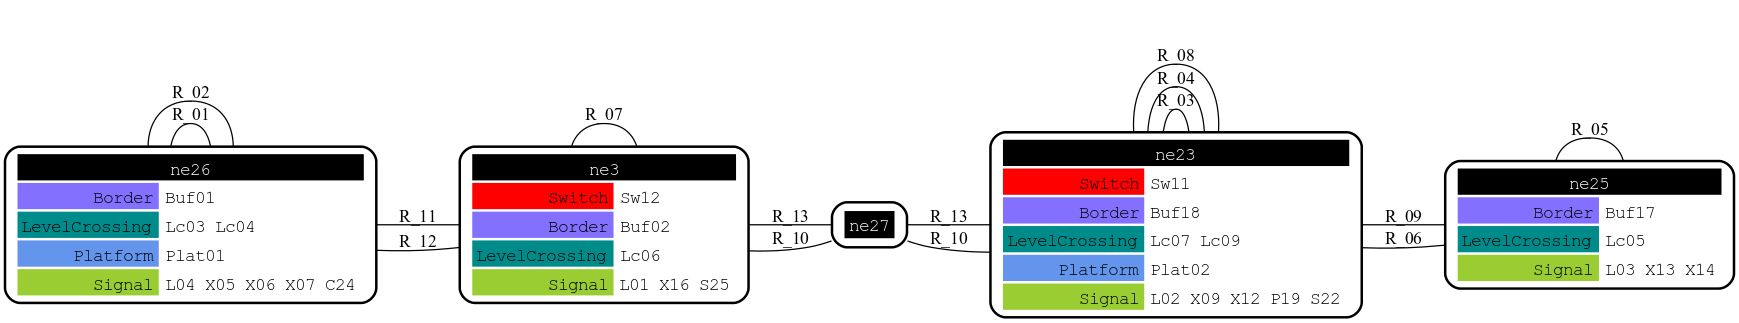
\includegraphics[width=1\textwidth]{Figuras/Graph_8}
    	\centering\caption{XXXX}
    	%\label{fig:LC_P2}
    \end{figure}
    
    \lipsum[1]

    \begin{figure}[h]
        \centering
        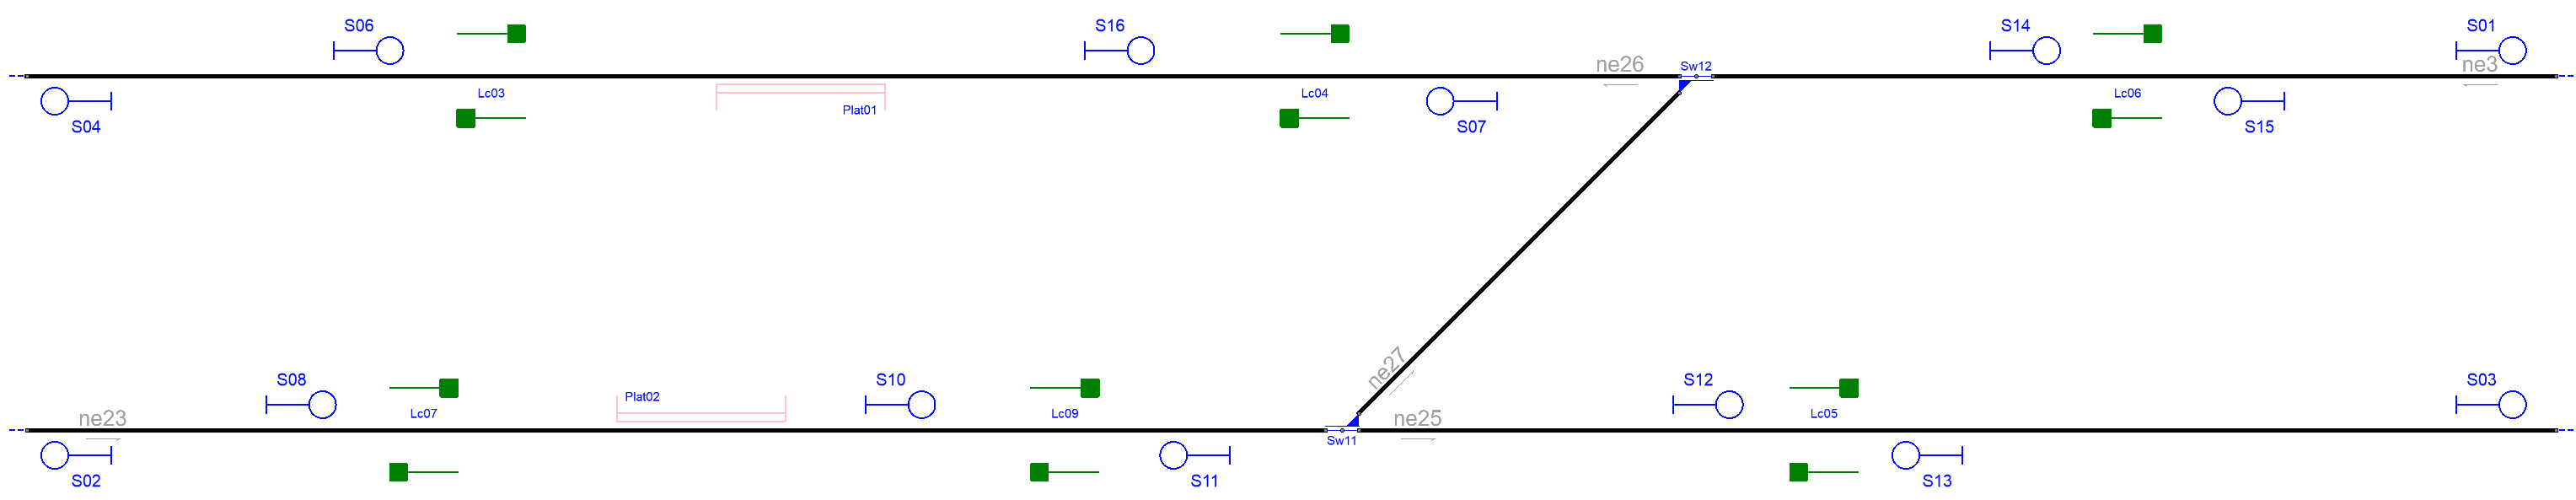
\includegraphics[width=1\textwidth]{resultados-obtenidos/ejemplo8/images/8_original.png}
        \centering\caption{Señalamiento original del ejemplo 8.}
        %\label{fig:LC_P2}
    \end{figure}

    \begin{figure}[h]
        \centering
        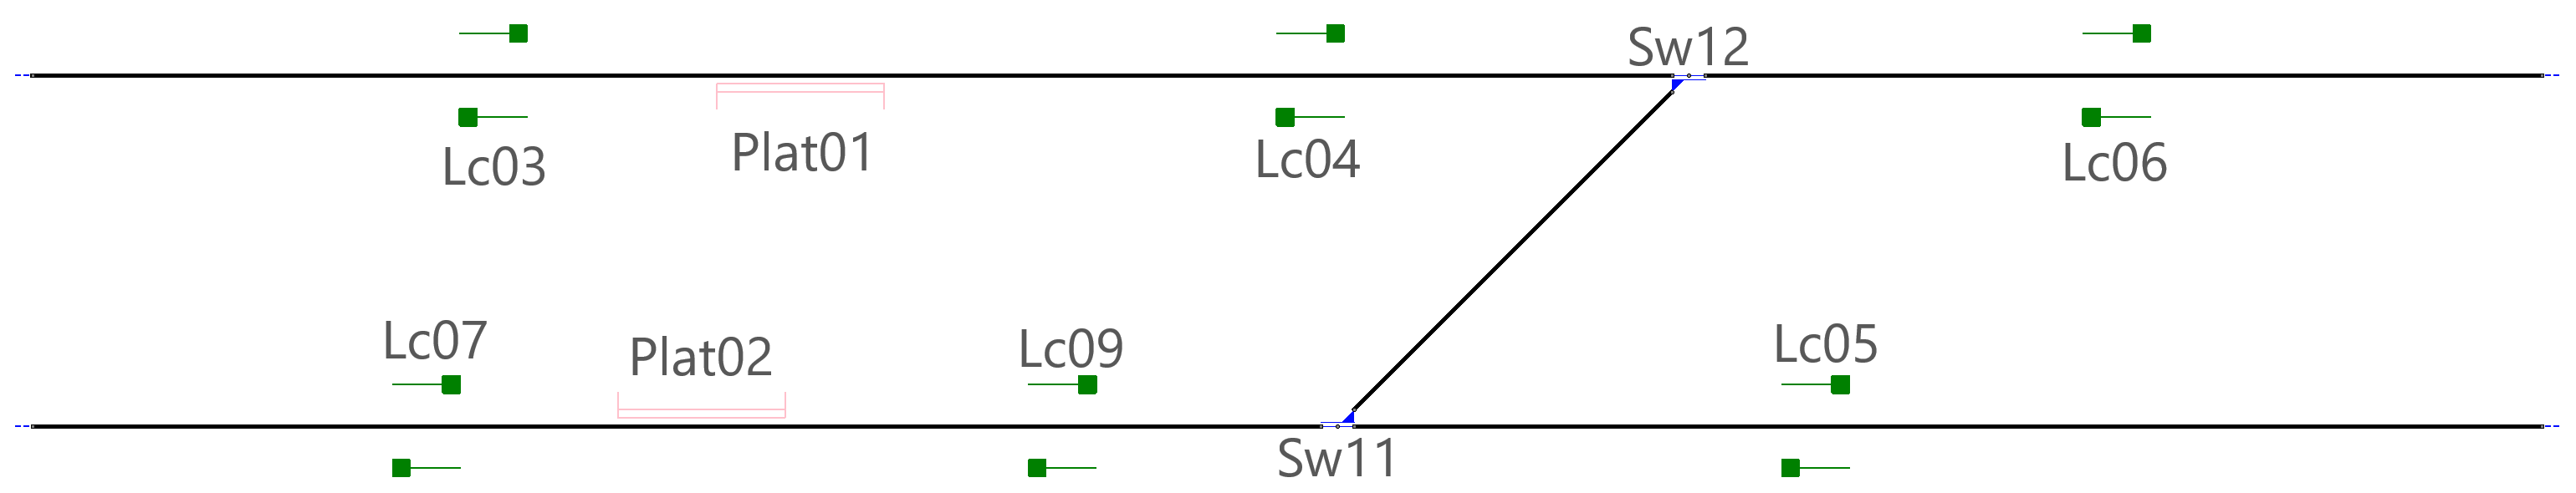
\includegraphics[width=1\textwidth]{resultados-obtenidos/ejemplo8/images/8_empty.png}
        \centering\caption{Topología ferroviaria del ejemplo 8 sin señalamiento.}
        %\label{fig:LC_P2}
    \end{figure}

    \begin{figure}[h]
        \centering
        
\includegraphics[width=1\textwidth]{resultados-obtenidos/ejemplo8/images/8_step1.png}
        \centering\caption{Señalamiento generado por el RNA para proteger el fín de vía.}
        %\label{fig:LC_P2}
    \end{figure}

    \begin{figure}[h]
        \centering
        
\includegraphics[width=1\textwidth]{resultados-obtenidos/ejemplo8/images/8_step2.png}
        \centering\caption{Señalamiento generado por el RNA para proteger las junturas.}
        %\label{fig:LC_P2}
    \end{figure}

    \begin{figure}[h]
        \centering
        
\includegraphics[width=1\textwidth]{resultados-obtenidos/ejemplo8/images/8_step3.png}
        \centering\caption{Señalamiento generado por el RNA para proteger plataformas y cruces de vía.}
        %\label{fig:LC_P2}
    \end{figure}

    \begin{figure}[h]
        \centering
        
\includegraphics[width=1\textwidth]{resultados-obtenidos/ejemplo8/images/8_step4.png}
        \centering\caption{Señalamiento generado por el RNA para proteger las máquinas de cambios.}
        %\label{fig:LC_P2}
    \end{figure}

    \begin{figure}[h]
        \centering
        
\includegraphics[width=1\textwidth]{resultados-obtenidos/ejemplo8/images/8_RNA.png}
        \centering\caption{Señalamiento generado y simplificado por el RNA.}
        %\label{fig:LC_P2}
    \end{figure}

    \subsection{Señalamiento original}

    \lipsum[1]
    
    \begin{table}[H]
        {
        \caption{Tabla de enclavamiento original del ejemplo 8.}
        \label{Tab:tabla_original_8}
        \centering
        \resizebox{1\textwidth}{!}{
            \begin{tabular}{ c c c c c c c }
                \hline	
                    Ruta & Inicio & Final & Cambio & Plataforma & Cruce & netElement \\	
                \hline
                    R$_{01}$  & S$_{06}$ & S$_{16}$ & - & Plat$_{01}$ & Lc$_{03}$ & ne$_{26}$\\
                    R$_{02}$  & S$_{07}$ & S$_{05}$ & - & Plat$_{01}$ & Lc$_{04}$ & ne$_{26}$\\
                    R$_{03}$  & S$_{08}$ & S$_{10}$ & - & Plat$_{02}$ & Lc$_{07}$ & ne$_{23}$\\
                    R$_{04}$  & S$_{10}$ & S$_{12}$ & Sw$_{11}^{N}$ & - & Lc$_{09}$ & ne$_{23}$-ne$_{25}$\\
                    R$_{05}$  & S$_{10}$ & S$_{14}$ & Sw$_{11}^{R}$+Sw$_{12}^{R}$ & - & Lc$_{09}$ & ne$_{23}$-ne$_{03}$\\
                    R$_{06}$  & S$_{11}$ & S$_{09}$ & - & Plat$_{02}$ & Lc$_{09}$ & ne$_{23}$\\
                    R$_{07}$  & S$_{12}$ & S$_{03}$ & - & - & Lc$_{05}$ & ne$_{25}$\\
                    R$_{08}$  & S$_{13}$ & S$_{11}$ & - & - & Lc$_{05}$ & ne$_{25}$-ne$_{23}$\\
                    R$_{09}$  & S$_{14}$ & S$_{01}$ & - & - & Lc$_{06}$ & ne$_{03}$\\
                    R$_{10}$  & S$_{15}$ & S$_{07}$ & Sw$_{12}^{N}$ & - & Lc$_{06}$ & ne$_{03}$-ne$_{26}$\\
                    R$_{11}$  & S$_{15}$ & S$_{11}$ & Sw$_{11}^{R}$+Sw$_{12}^{N}$ & - & Lc$_{06}$ & ne$_{03}$-ne$_{23}$\\
                    R$_{12}$  & S$_{16}$ & S$_{14}$ & - & - & Lc$_{04}$ & ne$_{26}$-ne$_{03}$\\
                \hline
            \end{tabular}
        }
     }
    \end{table}
    
    \lipsum[1]
    \section{Señalamiento generado por el RNA}

    El RNA también exporta la misma información mostrada en el Código \ref{lst:EJ8_8} en una hoja de cálculo, similar a la que se visualiza en la Tabla \ref{Tab:tabla_generated_8}.
    
    \begin{table}[H]
        {
        \caption{Tabla de enclavamiento del ejemplo 8 generada por el RNA.}
        \label{Tab:tabla_generated_8}
        %\centering
        \begin{center}      
        	\resizebox{0.8\textwidth}{!}{
            \begin{tabular}{ c c c c c c c }
                \hline	
                    Ruta & Inicio & Final & Cambio & Plataforma & Cruce & netElement \\	
                \hline
                    R$_{01}$  & X$_{05}$ & L$_{04}$ & - & - & Lc$_{03}$ & ne$_{26}$\\
                    R$_{02}$  & X$_{06}$ & C$_{24}$ & - & Plat$_{01}$ & Lc$_{03}$ & ne$_{26}$\\
                    R$_{03}$  & X$_{07}$ & X$_{05}$ & - & Plat$_{01}$ & Lc$_{04}$ & ne$_{26}$\\
                    R$_{04}$  & X$_{09}$ & S$_{22}$ & - & Plat$_{02}$ & Lc$_{07}$ & ne$_{23}$\\
                    R$_{05}$  & X$_{12}$ & P$_{19}$ & - & Plat$_{02}$ & Lc$_{09}$ & ne$_{23}$\\
                    R$_{06}$  & X$_{13}$ & L$_{03}$ & - & - & Lc$_{05}$ & ne$_{25}$\\
                    R$_{07}$  & X$_{14}$ & X$_{12}$ & Sw$_{11}^{N}$ & - & Lc$_{05}$ & ne$_{25}$-ne$_{23}$\\
                    R$_{08}$  & X$_{16}$ & L$_{01}$ & - & - & Lc$_{06}$ & ne$_{03}$\\
                    R$_{09}$  & P$_{19}$ & L$_{02}$ & - & - & Lc$_{07}$ & ne$_{23}$\\
                    R$_{10}$  & S$_{22}$ & X$_{13}$ & Sw$_{11}^{N}$ & - & Lc$_{09}$ & ne$_{23}$-ne$_{25}$\\
                    R$_{11}$  & S$_{22}$ & X$_{16}$ & Sw$_{11}^{R}$+Sw$_{12}^{R}$ & - & Lc$_{09}$ & ne$_{23}$-ne$_{03}$\\
                    R$_{12}$  & C$_{24}$ & X$_{16}$ & Sw$_{12}^{N}$ & - & Lc$_{04}$ & ne$_{26}$-ne$_{03}$\\
                    R$_{13}$  & S$_{25}$ & X$_{07}$ & Sw$_{12}^{N}$ & - & Lc$_{06}$ & ne$_{03}$-ne$_{26}$\\
                    R$_{14}$  & S$_{25}$ & X$_{12}$ & Sw$_{04}^{R}$+Sw$_{07}^{N}$ & - & Lc$_{06}$ & ne$_{03}$-ne$_{23}$\\
                \hline
            \end{tabular}
        }
        \end{center}
     }
    \end{table}
    
    En una primera inspección podemos ver que el nuevo señalamiento tiene 14 rutas, versus las 12 rutas del señalamiento original (ver Tabla \ref{Tab:tabla_original_8}). Esto se debe a que el RNA añadió paradas intermedias entre algunos elementos, dividiendo algunas rutas demasiado largas.
    \section{Sistema generado por el ACG}

	En base a la red de grafos, ilustrada en la Figura \ref{fig:EJ8_8}, el ACG determinó la siguiente cantidad de elementos, tal puede visualizarse en el Código \ref{lst:EJ8_8}.
	
	\begin{lstlisting}[language = {}, caption = Cantidad de elementos a implementar por el ACG, label = {lst:EJ8_8}]
	n_netElements:5
	n_switch:2
	n_doubleSwitch:0
	n_borders:4
	n_buffers:0
	n_levelCrossings:6
	n_platforms:2
	n_scissorCrossings:0
	n_signals:16
	N : 58
	M : 53
	\end{lstlisting}
	
	El código VHDL generado por el ACG es importado en un proyecto de Vivado, donde es sintetizado e implementado para generar el bitstream que será utilizado para programar la FPGA. La cantidad de elementos de la FPGA utilizados por el sistema post-síntesis y post-implementación, así como el porcentaje de uso de la plataforma, son detallados en la Tabla \ref{Tab:tabla_ACG_8}.
	
	\begin{table}[H]
		{
			\caption{Síntesis e implementación del ejemplo 8 generado por el ACG.}
			\label{Tab:tabla_ACG_8}
			\centering
			%\small
			%\centering
			\begin{center}
				\resizebox{0.7\textwidth}{!}{
					\begin{tabular}{ c c c c }
						\hline	
						Recursos & Síntesis & Implementación & Uso \\	
						\hline
						LUT & 2786 & 2784 & 5.24-5.23\%\\
						FF & 3848 & 3848 & 3.62\%\\
						IO & 16 & 16 & 12.80\%\\
						BUFG & 1 & 1 & 3.13\%\\
						\hline
					\end{tabular}
				}
			\end{center}
		}    
	\end{table}
	
	En este ejemplo, la cantidad de recursos utilizados es baja y el tiempo de sintetización e implementación es de 37 segundos y 38 segundos respectivamente.
    \subsection{Validacion del sistema}

    Las 12 rutas del señalamiento original (Tabla \ref{Tab:tabla_original_8}) tienen 12 rutas equivalentes en el señalamiento generado por el RNA (Tabla \ref{Tab:tabla_generated_8}), tal como se puede visualizar en la Tabla \ref{Tab:tabla_validation_8}, generada automáticamente por el RNA.

    \begin{table}[H]
        {
        \caption{Equivalencias entre las rutas originales y las generadas por el RNA.}
        \label{Tab:tabla_validation_8}
        \centering
        %\small
            %\centering
            \begin{center}
            \resizebox{0.7\textwidth}{!}{
            \begin{tabular}{ c c c c }
                \hline	
                    Original & Señales & RNA & Señales \\	
                \hline
                    R$_{01}$ & S$_{06}$-S$_{16}$ & R$_{02}$ & X$_{06}$-C$_{24}$ \\
                    R$_{02}$ & S$_{07}$-S$_{05}$ & R$_{03}$ & X$_{07}$-X$_{05}$ \\
                    R$_{03}$ & S$_{08}$-S$_{10}$ & R$_{04}$ & X$_{09}$-S$_{22}$ \\
                    R$_{04}$ & S$_{10}$-S$_{12}$ & R$_{10}$ & S$_{22}$-X$_{13}$ \\
                    R$_{05}$ & S$_{10}$-S$_{14}$ & R$_{11}$ & S$_{22}$-X$_{16}$ \\
                    R$_{06}$ & S$_{11}$-S$_{09}$ & R$_{09}$ & P$_{19}$-L$_{02}$ \\
                    R$_{07}$ & S$_{12}$-S$_{03}$ & R$_{06}$ & X$_{13}$-L$_{03}$ \\
                    R$_{08}$ & S$_{13}$-S$_{11}$ & R$_{07}$ & X$_{14}$-X$_{12}$ \\
                    R$_{09}$ & S$_{14}$-S$_{01}$ & R$_{08}$ & X$_{16}$-L$_{01}$ \\
                    R$_{10}$ & S$_{15}$-S$_{07}$ & R$_{13}$ & S$_{25}$-X$_{07}$ \\
                    R$_{11}$ & S$_{15}$-S$_{11}$ & R$_{14}$ & S$_{25}$-X$_{12}$ \\
                    R$_{12}$ & S$_{16}$-S$_{14}$ & R$_{12}$ & C$_{24}$-X$_{16}$ \\
                \hline
            \end{tabular}
            }
            \end{center}
        }    
    \end{table}
    
    Las rutas R1 y R5 (Tabla \ref{Tab:tabla_generated_1}) generadas por el RNA que no tienen equivalencias en el señalamiento original (Tabla \ref{Tab:tabla_original_1}) se deben a que el RNA creó señales extras. La ruta R1 es definida por el RNA al crear la señal X05 entre la plata forma Plat01 y el cruce de vías Lc03, lo cual genera una parada intermedia que antes no existía, hasta culminar la ruta en la señal L04. De la misma manera, el RNA define la ruta R5 al crear la señal P19, lo cual genera una parada intermedia entre la platforma Plat02 y el cruce de vías Lc07. En definitiva, el RNA dividió las rutas R2 y R6 originales en las nuevas rutas R3+R1 y R5+R9. Lo cual mejora la logística de la red ferroviaria.